\documentclass[12pt,a4paper]{article}

\usepackage[swedish]{babel}
\usepackage[margin=1in,includefoot]{geometry} 
\usepackage{graphicx}
\usepackage{float}
\usepackage[format=plain,labelfont=it]{caption}
\usepackage[backend=bibtex,style=authoryear,citestyle=authoryear-comp]{biblatex}
\usepackage[bottom]{footmisc}
\bibliography{./references/etthundra.bib}

\begin{document}

  \begin{titlepage}
    \begin{center} 
      \begin{huge}
        \textsc{Maskininlärning och tärningsspelet \emph{Etthundra}} \\ 
        \vspace{0.75cm} 
      \end{huge} 
      \large{En undersökning kring huruvida en maskinintelligens kan bli konsekvent bättre än människor på tärningsspelet \emph{Etthundra}} 
    \end{center}

    \vspace{\fill} 
    \begin{flushleft} 
      \textbf{Elever:} REDACTED
      \textbf{Program:} REDACTED
      \textbf{Klass:} REDACTED
      \textbf{Handledare:} REDACTED
      \textbf{Datum:} 2020-03-08
    \end{flushleft}
  \end{titlepage}
  
  \pagenumbering{roman} 

  \section*{Sammanfattning}\label{sec:samanfattning}
    \addcontentsline{toc}{section}{\numberline{}Sammanfattning}
    Syftet med denna undersökning är att studera ifall en maskinintelligens som tränats med Q-learning metoden konsekvent kan vinna över människor på tärningsspelet \emph{Etthundra}. Q-learning metoden baseras på straff och belöningar, där maskinintelligensen straffas vid drag som inte leder till en vinst och belönas för dem som gör det. Maskinintelligensen programmerades i Python och fick träna \emph{20 miljoner} spel. Den testades sedan både mot människor och andra, mindre tränade maskinintelligenser. Resultaten visar att maskinintelligensen inte blivit bättre än människor, dock tyder resultatet på att maskinintelligensen presterar bättre efter träning.

  \section*{Abstract}\label{sec:abstract}
    \addcontentsline{toc}{section}{\numberline{}Abstract} 
    The purpose of this study is to investigate whether or not a machine intelligence that has been trained according to the Q-learning method consistently can defeat humans in the dice game \emph{Etthundra}. The Q-learning method is based on punishment and reward. If the machine intelligence makes moves that results in a win, the machine intelligence gets rewarded, otherwise it gets punished. The machine intelligence was programmed in Python and got to train \emph{20 million} games. It was then tested against both humans and other, less-trained machine intelligences. The results show that the machine intelligence can not consistently beat humans. However, the results indicate that the machine intelligence performs better after training.

  \cleardoublepage

  \thispagestyle{empty} 
  \tableofcontents 

  \cleardoublepage

  \pagenumbering{arabic}

  \section{Inledning}\label{sec:inledning}
    \subsection{Bakgrund}\label{subsec:bakgrund} 
      Överallt i samhället går det att finna maskinintelligenser. Användningsområdena är många och innefattar allt från smarta röstassistenter till självkörande bilar. Dock finns många sektorer där maskinintelligens ännu inte tillämpats och därav är kunskap inom maskinintelligens mycket attraktivt på arbetsmarknaden och inom en snar framtid kan maskinintelligens komma att förbättra vår vardag ännu mer. \footcite{ref:stackoverflowai}

      Ett tidigare nämnt användningsområde är självkörande bilar, som skulle kunna medföra att Sverige når nollvisionen. Ett annat användningsområde är inom medicin. Maskinintelligenser används redan idag för att assistera doktorer vid diagnostisering av diverse sjukdomar och tillstånd, bland annat cancer. \footcite{ref:cancer} Dessutom skulle en maskinintelligens kunna finna nya kemiska föreningar som potentiellt skulle kunna användas för att bota tidigare obotliga sjukdomar. \footcite{ref:antibiotika} Ännu ett tillämpningsområde är miljön. En maskinintelligens skulle kunna uppfinna nya, effektivare förbränningsmotorer som belastar miljön mindre, eller optimera redan existerande motorer och på så sätt hjälpa mänskligheten nå klimatmålen. \footcite{ref:motorer}

    \subsection{Syfte}\label{subsec:syfte} 
      Syftet med detta gymnasiearbete är att programmera maskinintelligenser och att sedan träna dem med hjälp av Q-learning. Detta för att undersöka om maskinintelligenserna konsekvent kan besegra människor i tärningsspelet \emph{Etthundra}.

    \subsection{Frågeställning}\label{subsec:fragestallning} 
      Går det att med hjälp av maskininlärning träna maskinintelligenser till att bli bättre än människor på tärningsspelet \emph{Etthundra}?

    \subsection{Avgränsningar}\label{subsec:avgransningar} 
      Denna rapport kommer endast att avhandla maskininlärningsmetoden Q-learning applicerat på tärningsspelet \emph{Etthundra}, även om det finns andra mer effektiva modeller.
    
  \cleardoublepage

  \section{Teori}\label{sec:teori}
    \subsection{\emph{Etthundra}}\label{subsec:etthundra} 
      Tärningsspelet \emph{Etthundra} spelas av två spelare, vars mål är att vara den som först samlar ihop 100 poäng. Detta utförs genom att spelarna turas om att slå tärningen. När det blir en spelares tur får den slå med tärningen, och den poäng som tärningen visar adderas till  spelarens så kallade temporära poäng. Spelaren får sedan fortsätta att slå med tärningen så länge den behagar, eller tills spelaren slår en etta. I fallet då spelaren väljer att avsluta sin tur överförs spelarens temporära poäng till dess permanenta poäng. Därefter nollställs de temporära poängen och turen går över till den andra spelaren. I det andra fallet, då spelaren slår en etta, adderas inte spelarens temporära poäng till dess permanenta poäng utan de temporära poängen nollställs och turen går sedan direkt över till den andra spelaren. Detta fortsätter tills någon av spelarnas permanenta poäng tangerar eller överskrider 100 poäng.

    \subsection{Maskininlärning}\label{subsec:maskininlarning} 
      Maskininlärning är ett samlingsord för hur datorer, med hjälp av olika inlärningsmetoder, kan lära sig att lösa en viss uppgift utan att den som programmerar metoden behöver kunna lösa uppgiften. Skillnaden mellan maskininlärning och konventionell artificiell intelligens är att den sistnämnda löser uppgiften baserat på kodad logik istället för att lära sig själv. När uppgiften som ska lösas innehåller få variabler är det oftast enklare att låta datorn lösa uppgiften med hjälp av logik programmerad av en människa. När uppgiften som ska lösas innehåller många variabler kan det vara fördelaktigt att använda sig av maskininlärning. Ett exempel som innehåller många variabler och därmed löses enklast med maskininlärning, är självkörande bilar. Att förklara för en dator hur man kör en bil med hjälp av programmerad logik är i princip omöjligt, bilkörning är för nyanserat. För att förstå komplexiteten med bilkörning kan ett exempel innehållande en korsning med en ljussignal uppdagas. Du ska svänga till vänster i korsningen och väntar på grön signal. Ljussignalen blir grön men bilen framför dig kör inte direkt och du måste därav vänta. När bilen framför väl kör, kan du inte svänga till vänster direkt eftersom bilarna som kör mot dig från andra sidan även har grönt och du måste vänta på att alla bilarna passerar innan du kan köra vidare. När bilarna har passerat kan du fortsätta din vänstersväng men måste ännu en gång stanna på grund av ett övergångsställe med fotgängare. Bevisligen erhåller en vänstersväng flertalet variabler och att programmera logik som kör en bil hade därför varit omöjligt. Istället använder man sig av maskininlärning. Genom att samla in data om hur man kör bil med hjälp av bland annat kameror, kan en dator sedan få analysera denna data och försöka att själv dra slutsatser kring hur man kör bil. Datorns slutsatser kring detta kan sedan testas i simulationer och utvärderas för att göra datorn bättre på att köra bil. 
      
      Även om maskininlärning brukar användas till stora och komplicerade problem går det att applicera denna inlärningsmetod på relativt lätta och små problem, däribland tärningsspelet \emph{Etthundra}. 

      \subsubsection{Q-learning}\label{subsubsec:qlearning} 
        Q-learning är en maskininlärningsmetod som baseras på positiv och negativ förstärkning. Datorn tillåts försöka lösa en uppgift och blir efter försöket belönad eller bestraffad. Om datorn löste uppgiften, eller ett delmål till uppgiften, blir den belönad. Om datorn inte löste uppgiften, eller om dess utfall handlingen gav upphov till anses vara dåligt, blir den bestraffad. Datorn kommer sedan ihåg belöningen eller bestraffningen och associerar denna med det sätt den försökte lösa uppgiften på just denna gång. Processen innefattade ett försök som leder till bestraffning eller belöning och sedan associering kallas att datorn tränar, vilket den gör tills att uppgiften anses vara löst på ett tillfredsställande sätt. I början av träningen slumpar datorn i princip alla sina drag, men gradvis under träningens gång baseras fler och fler av datorns val på den kunskap den samlat. Hur snabbt denna stegringen sker bestäms av ett $\varepsilon$-värde. Högt $\varepsilon$ leder till en långsammare stegring, lågt $\varepsilon$ leder till en snabbare stegring. Denna stegringen finns för att datorn ska utforska många olika kombinationer av drag och inte anta att det bästa sättet att utföra uppgiften på är det sätt som skedde vid första försöket.
        
        Hur datorn kommer ihåg om ett drag är bra eller dåligt är genom en tabell, ett Q-table. På vänster sida av tabellen finns varje giltig position i spelet \emph{Etthundra} och överst finns de möjliga dragen, att slå eller att stanna. Varje kombination av position och drag blir graderade med en siffra baserat på hur gynnsamt draget är att utföra från just denna positionen. För exempel, se bilaga \ref{tab:qtable}. Att beräkna denna gradering, och då siffra, är enkelt om draget leder till en belöning eller en bestraffning. Värdet av siffran blir då bara det värde som associeras med en belöning respektive bestraffning, exempelvis 100 respektive $-100$. För att beräkna värdet av siffran för en kombination av position och drag som inte direkt leder till en belöning eller bestraffning används en SARSA-algoritm. Med hjälp av denna kan värdet för siffran beräknas då algoritmen tar hänsyn till om ett drag i framtiden leder till en belöning eller bestraffning. Detta eftersom ett drag som leder till ett drag som ger belöning är bättre än ett drag som leder till ett drag som inte ger belöning, eller värre, en bestraffning. När datorn har tränat färdigt och den bes spela \emph{Etthundra}, observerar den enbart vilken position som spelet är i inför varje slag och väljer sedan det drag med högst associerat värde. Se bilaga \ref{tab:qtable} för exempel.

      \subsubsection{Maskininlärning och tärningsspelet \emph{Etthundra}}\label{subsubsec:maskininlarningochtarningsspeletetthundra} 
        Antalet giltiga positioner i \emph{Etthundra} är ungefär 500 000. Varje spelare kan besitta en poäng mellan 0 och 100 och en temporär poäng mellan 0 till 100. Detta leder till att antalet giltiga positioner är $100^3 = 1 000 000$. Dock halveras antalet positioner eftersom en spelare som erhåller 60 poäng inte behöver slå mer än 40 poäng på en runda. Därav finns det ungefär 500 000 giltiga positioner och dimensionen av Q-tablet är därför ungefär: 500 000 positioner x 2 drag.

      \subsubsection{SARSA}\label{subsubsec:sarsa} 
        Värdet för en kombination av position och drag Q, beräknas med hjälp av SARSA-algoritmen:

        \begin{eqnarray}\label{eqn:sarsa} 
          Q(S, A) \leftarrow Q(S, A) + \alpha(R + \gamma \cdot Q(S’, A’) - Q(S, A) 
        \end{eqnarray}

        Där $S$ betecknar position (engelska state), $A$ står för drag (engelska action), $R$ för värdet av belöning/bestraffning (engelska reward), $S’$ för nästa position och $A’$ för nästa drag. Variabeln $\alpha$ bestämmer hur mycket värdet $Q$ förändras av ny information. Variabeln $\gamma$ bestämmer hur mycket värdet $Q$ ska baseras på framtida belöningar/bestraffningar.

    \subsection{Python}\label{subsec:python} 
      Programmeringsspråket Python är väl lämpat för maskininlärning. Detta då Python är mycket modulärt, d.v.s det finns många färdigskrivna bibliotek med kod som man lätt kan implementera i sina egna program. Detta gör det mycket lätt att implementera svåra och avancerade koncept kopplade till maskininlärning med få rader kod. 
      
      Python är också väldigt användarvänligt då språket är väldigt likt engelskan, vilket gör att många lär sig Python som sitt första programmeringsspråk. Detta har gjort Python till ett av de mest använda programmeringsspråken vilket underlättar vid problemsituationer eftersom lösningen på problemet antagligen går att finna på internetforum. \footcite{ref:stackoverflow}

      Dessa anledningar gör Python till det självklara valet när man ska programmera och träna maskinintelligenser.
    
    \subsection{Materiel}\label{subsec:materiel} 
      En dator med Python 3.7 installerat.
    
    \subsection{Metod}\label{subsec:metod}
      \subsubsection{Maskinintelligens mot människor}\label{subsubsec:maskinintelligensmotmanniskor} 
        För att undersöka hur bra maskinintelligenserna presterade gentemot människor fick ett antal personer möta dem. Varje person fick spelet \emph{Etthundra} förklarat för sig, därefter fick de börja spela mot en förutbestämd nivå av maskinintelligensen. Totalt testades fyra nivåer av maskinintelligensen: \emph{100} (\emph{nivå 1}), \emph{5 miljoner} (\emph{nivå 2}), \emph{10 miljoner} (\emph{nivå 3}) och slutligen \emph{20 miljoner} (\emph{nivå 4}) tränade spel. De som mötte datorn spelade varannan runda som spelare ett och varannan runda som spelare två. Totalt spelade varje person fyra spel. Efter varje färdigspelat spel antecknades resultatet.

      \subsubsection{Maskinintelligens mot maskinintelligens}\label{subsubsec:maskinintelligensmotmaskinintelligens} 
        För att analysera om maskinintelligensen blivit bättre, fick den mest tränade maskinintelligensen, \emph{nivå 4}, möta: \emph{nivå 1}, \emph{nivå 2} och \emph{nivå 3}. Under en match spelades 3000 spel. Totalt genomfördes 9000 spel mellan den mest tränade maskinintelligensen, \emph{nivå 4}, och de olika träningsnivåerna. Resultaten antecknades efter varje färdigspelad match.

  \section{Utförande}\label{sec:utforande} 
    Undersökningen startade med att en maskinintelligens programmerades utifrån Q-learning modellen, se \ref{subsubsec:qlearning}. Denna modellen baserades på SARSA ekvationen, se ekvation \ref{eqn:sarsa}.
    
    Därefter fick två instanser av maskinintelligensen träna mot varandra tills de spelat totalt \emph{20 miljoner} spel. Under tiden de tränade sparades maskinintelligensens utveckling med jämna intervaller, för att möjliggöra undersökning av dess utveckling.

    Sedan testades instanserna mot både människor och mot varandra, se \ref{subsec:metod}. Resultaten registrerades i CSV-format, se bilaga \ref{app:data}.

    Resultaten sammanfördes i enkla grafer vilka förenklade analysen.

  \section{Resultat}\label{sec:resultat} 
    När människor mötte maskinintelligens \emph{nivå 1} vann människorna 100\% av spelen. Respektive värde för maskinintelligens av \emph{nivå 2}, \emph{nivå 3} och \emph{nivå 4} är 95,8\%, 100\% samt 92,9\%, se figur \ref{fig:vinstandelmanniskor}. Under dessa spelen uppnådde maskinintelligens \emph{nivå 1} i genomsnitt 38,4 poäng, lägre än vad de andra nivåerna presterade. Dessa uppnådde istället en medelpoäng mellan 53 och 59 poäng, se \emph{figur \ref{fig:medelpoangmaskinintelligens}}. När maskinintelligensen \emph{nivå 4} mötte maskinintelligenserna av \emph{nivå 1} och \emph{nivå 3} vann den en majoritet av spelen. Dock så förlorade den majoriteten av spelen när den mötte maskinintelligensen \emph{nivå 2}, se figur \ref{fig:vinstandelniva4}. För all data som tabellerna baseras på, se bilaga \ref{app:data}.
    
    \begin{figure}[H]
      \centering
      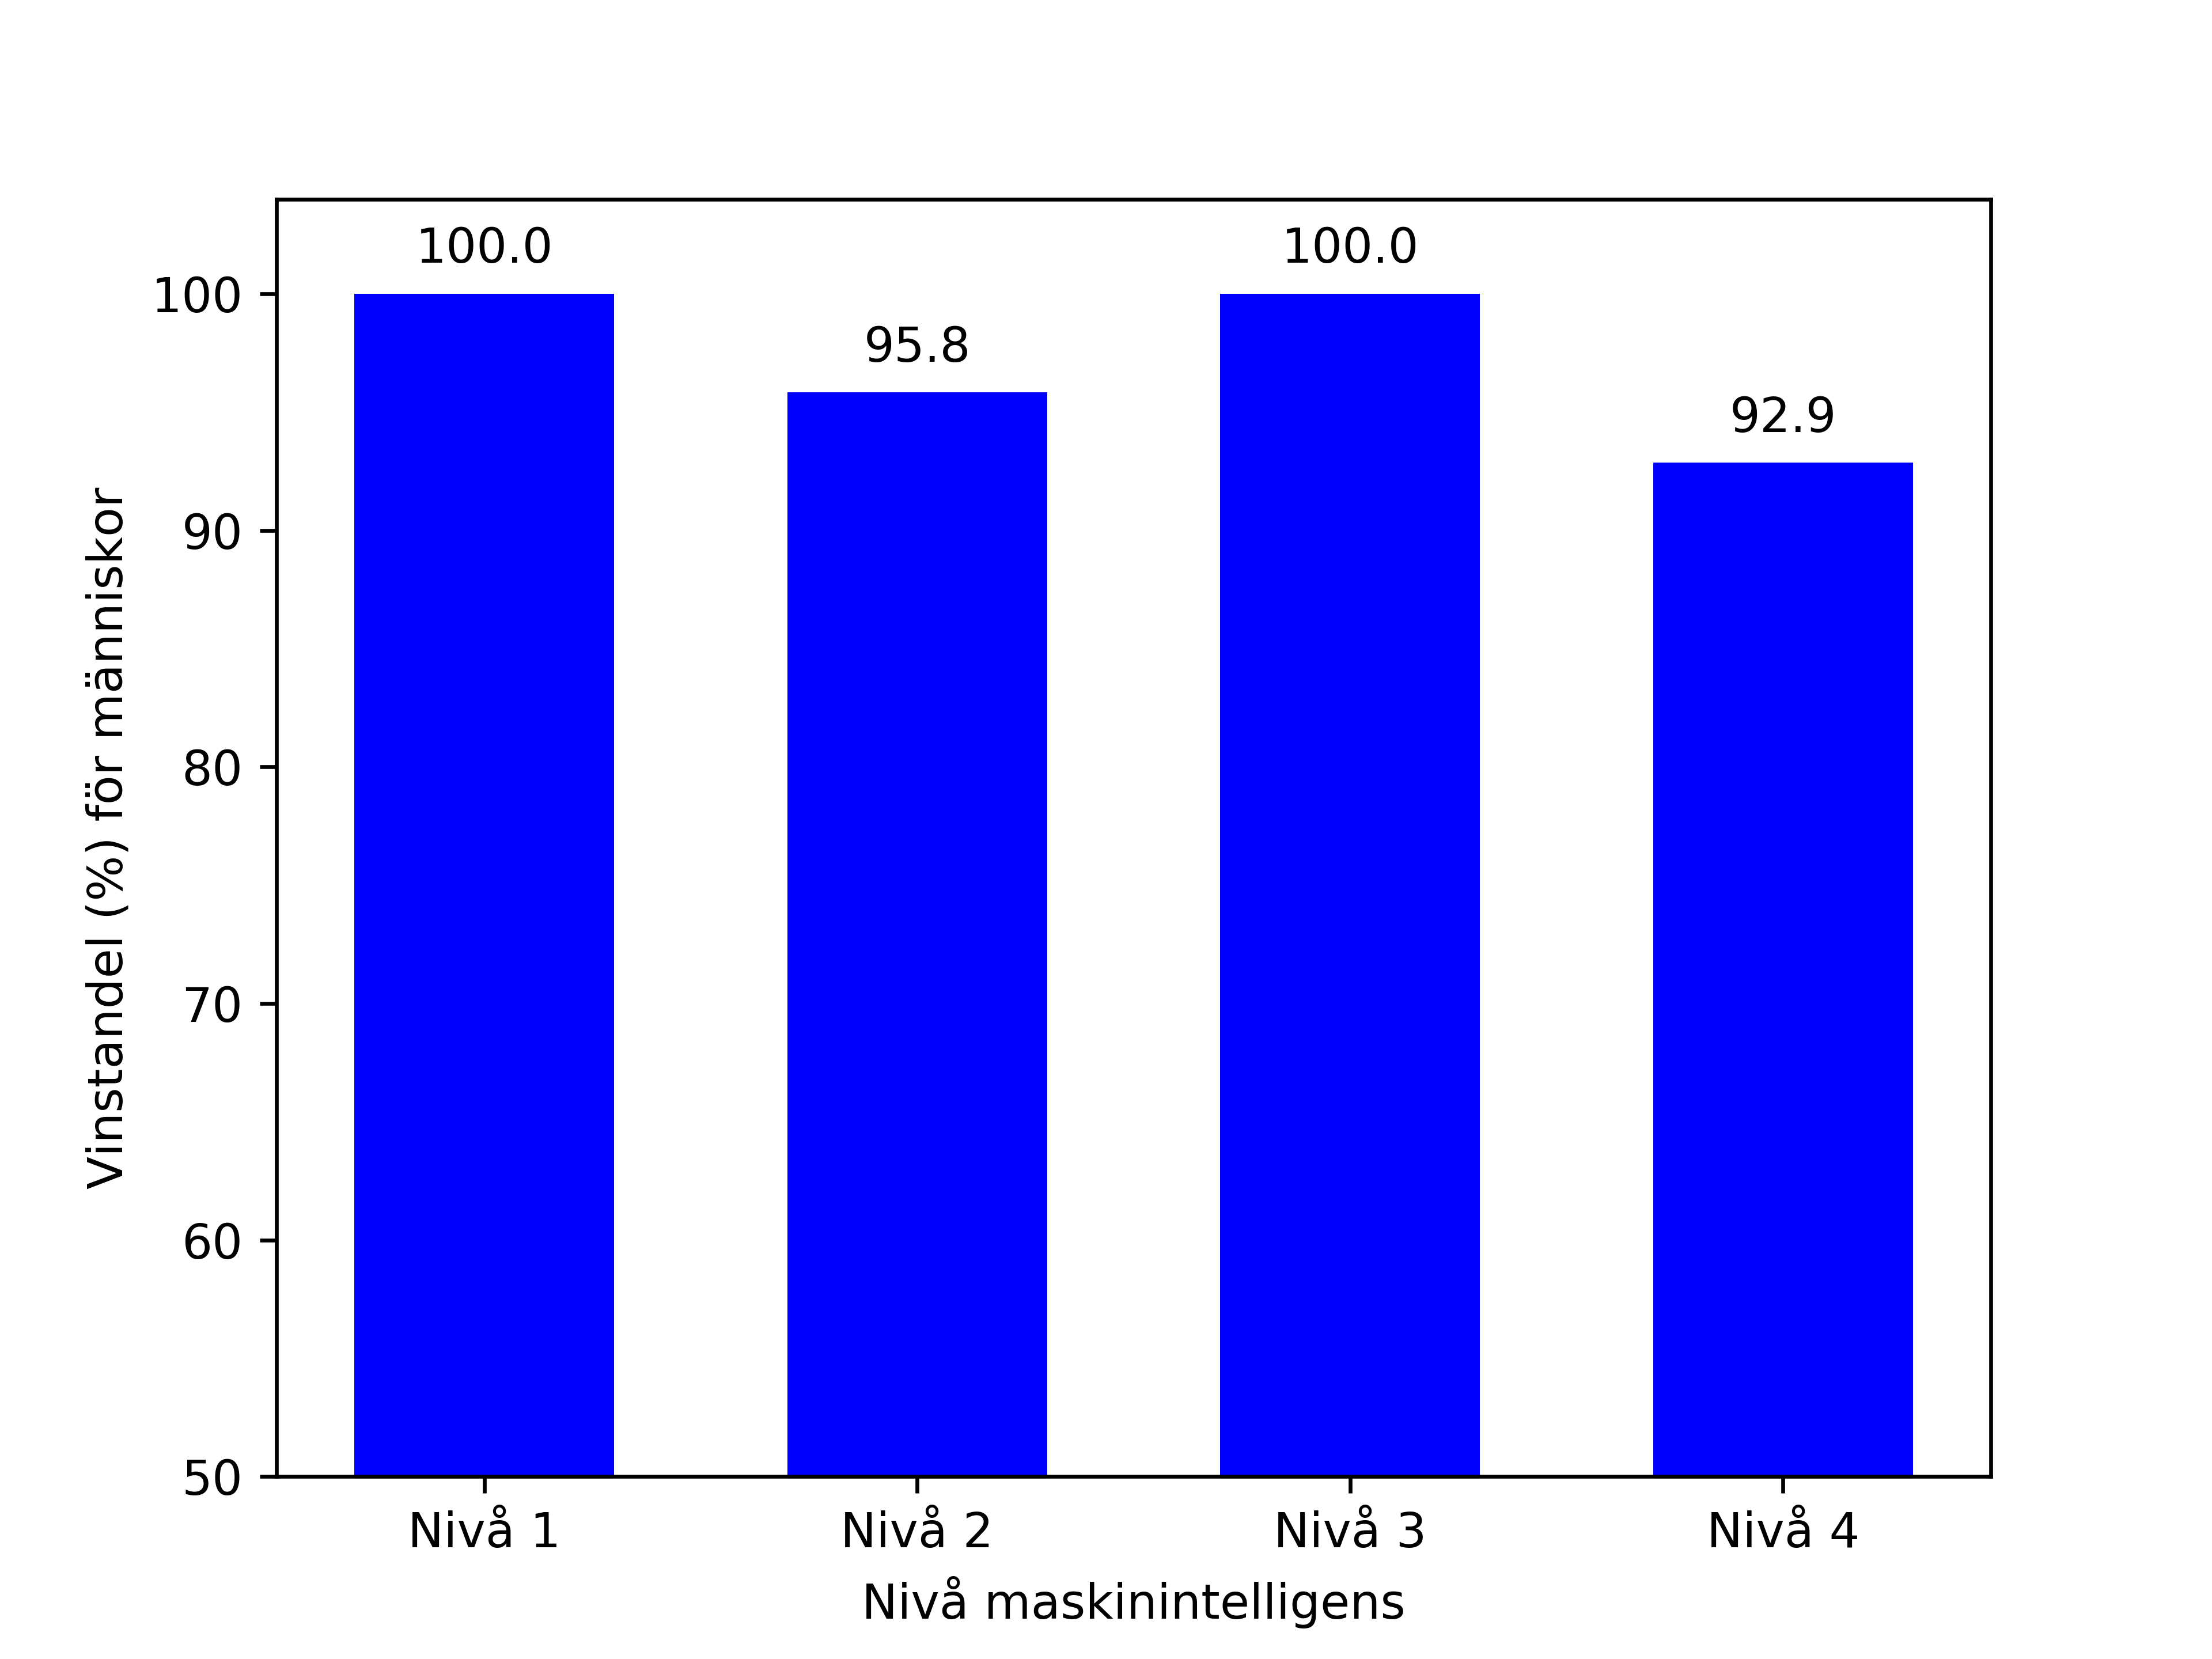
\includegraphics[height=3.5in]{./images/vinstandel_manniskor.png}
      \caption{Figuren visar på hur stor andel av genomförda spel som människa vinner mot maskinintelligens av en given nivå.}
      \label{fig:vinstandelmanniskor} 
    \end{figure}
    
    \begin{figure}[H] 
      \centering
      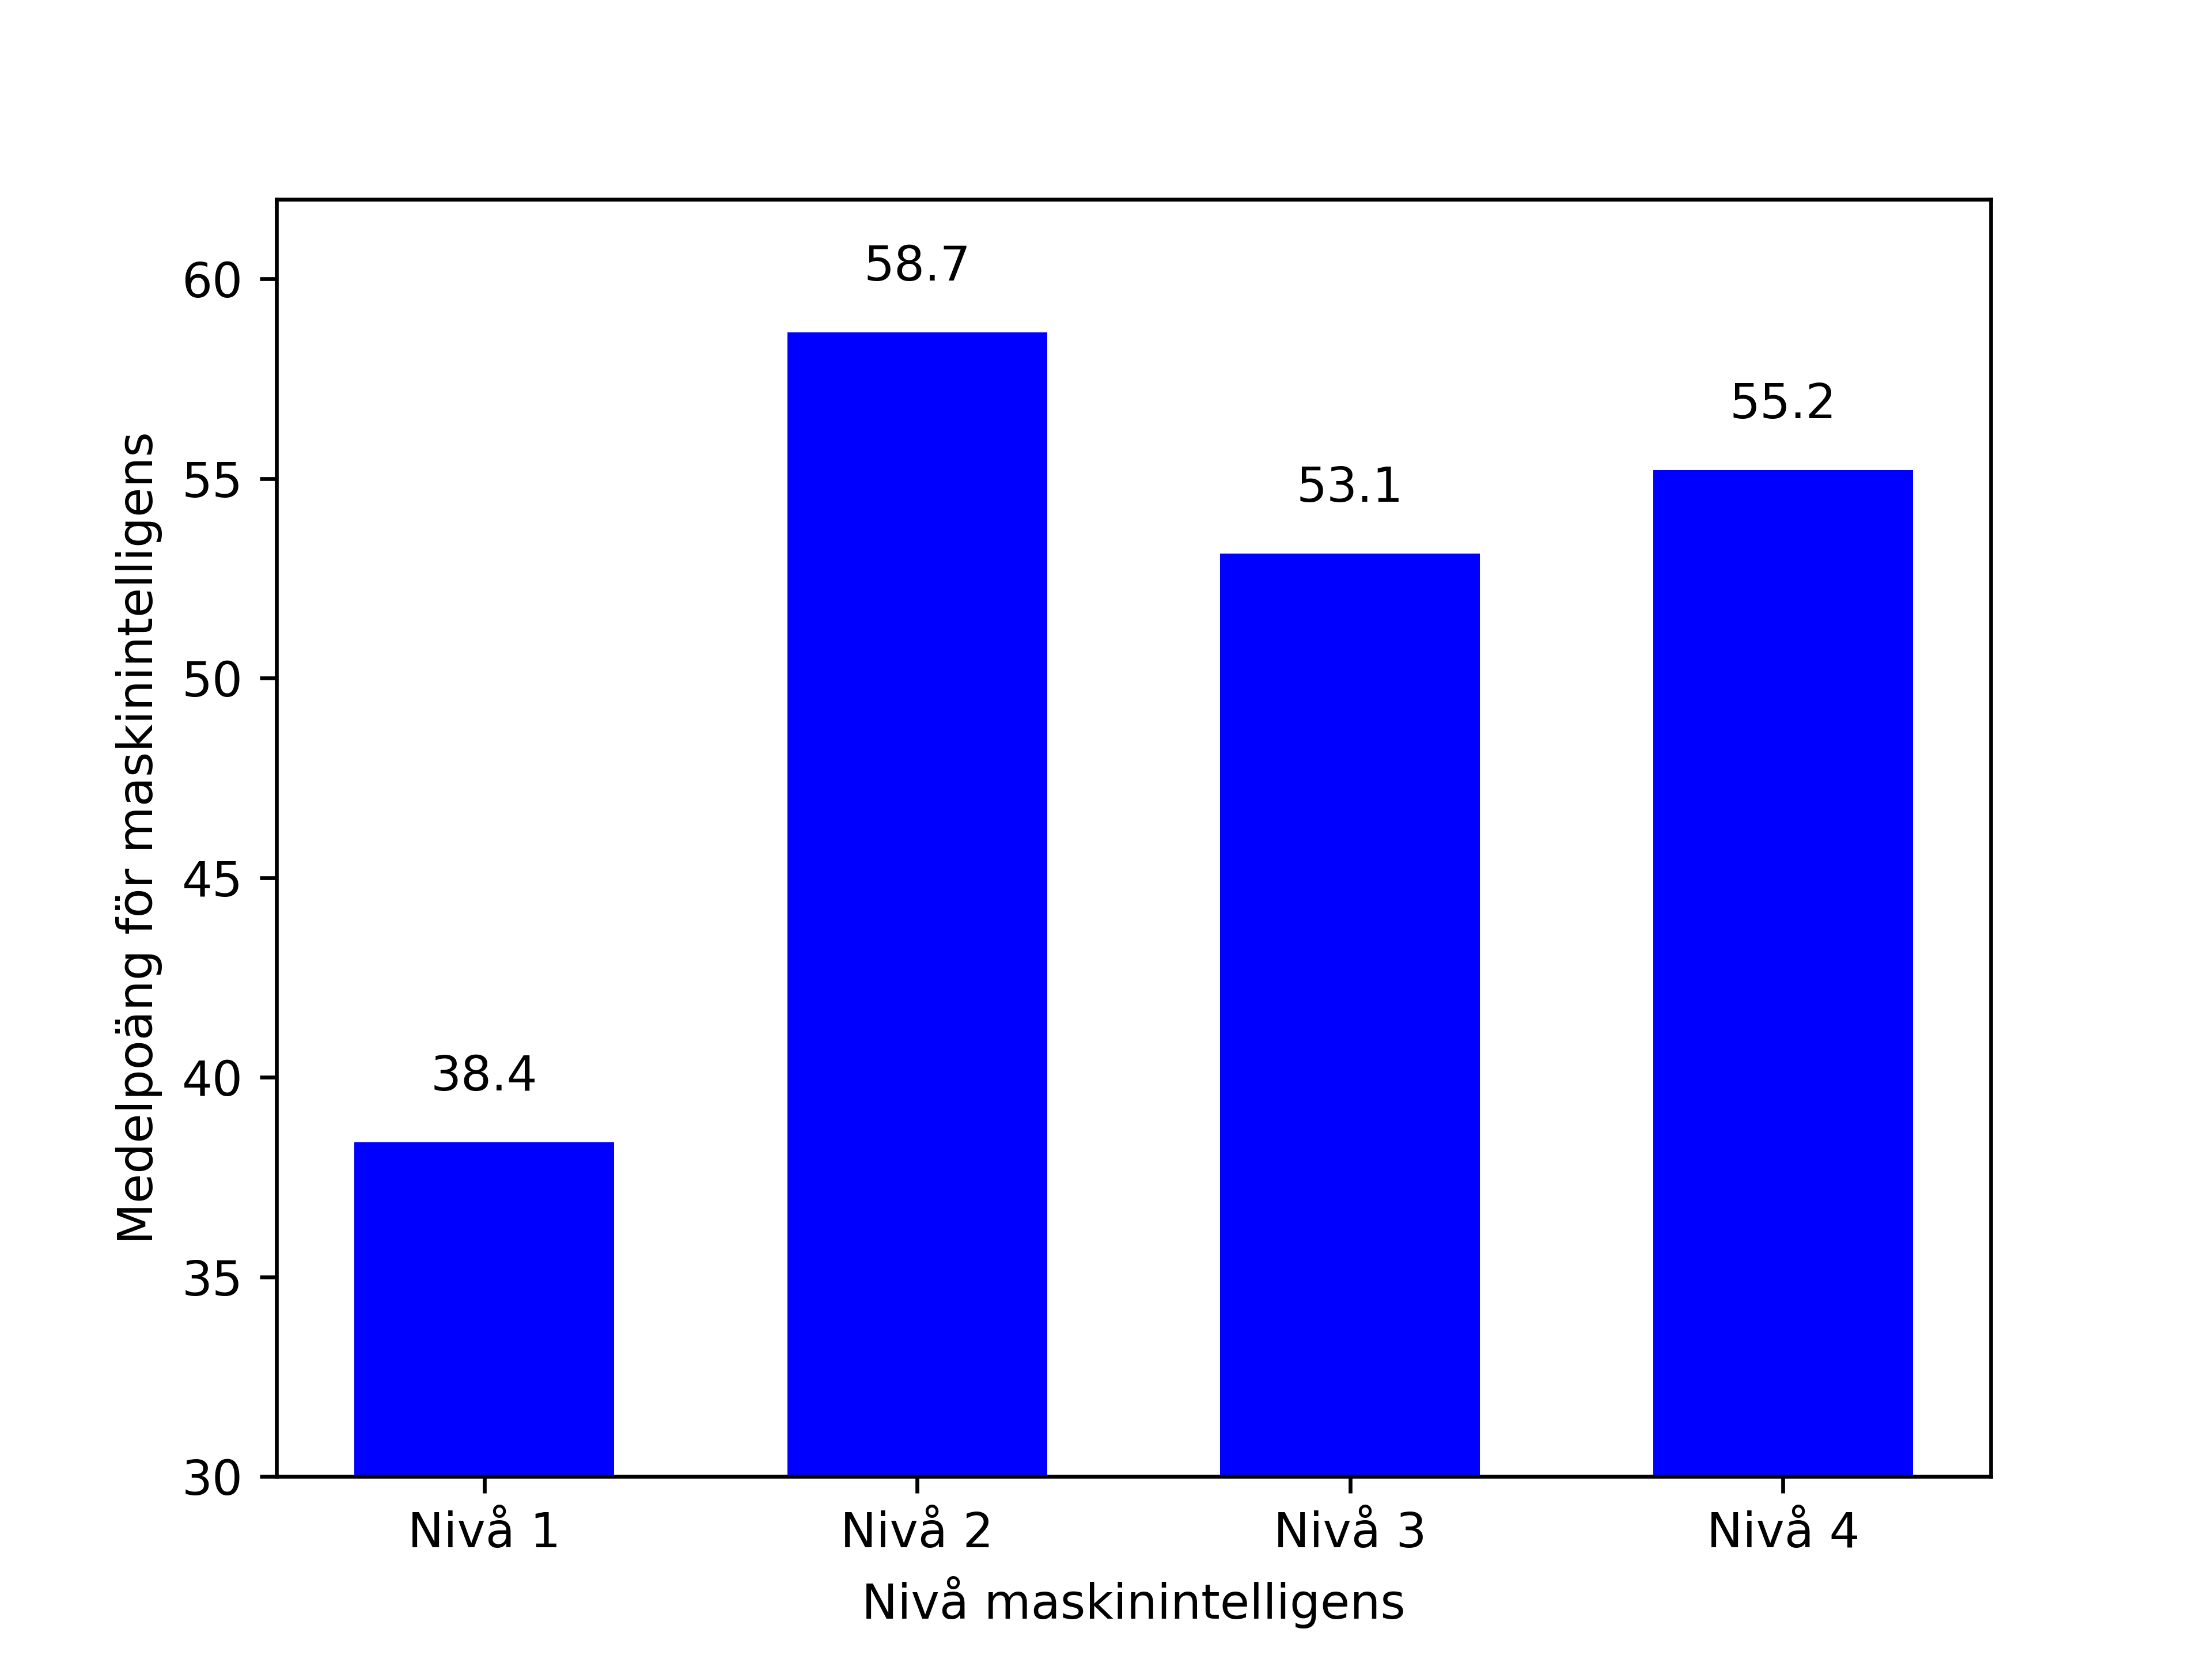
\includegraphics[height=3.5in]{./images/medelpoang_maskinintelligens.png}
      \caption{Figuren visar medelpoängen för en maskinintelligens av en viss nivå då den mötte människor.}
      \label{fig:medelpoangmaskinintelligens}
    \end{figure}

    \begin{figure}[H] \centering
      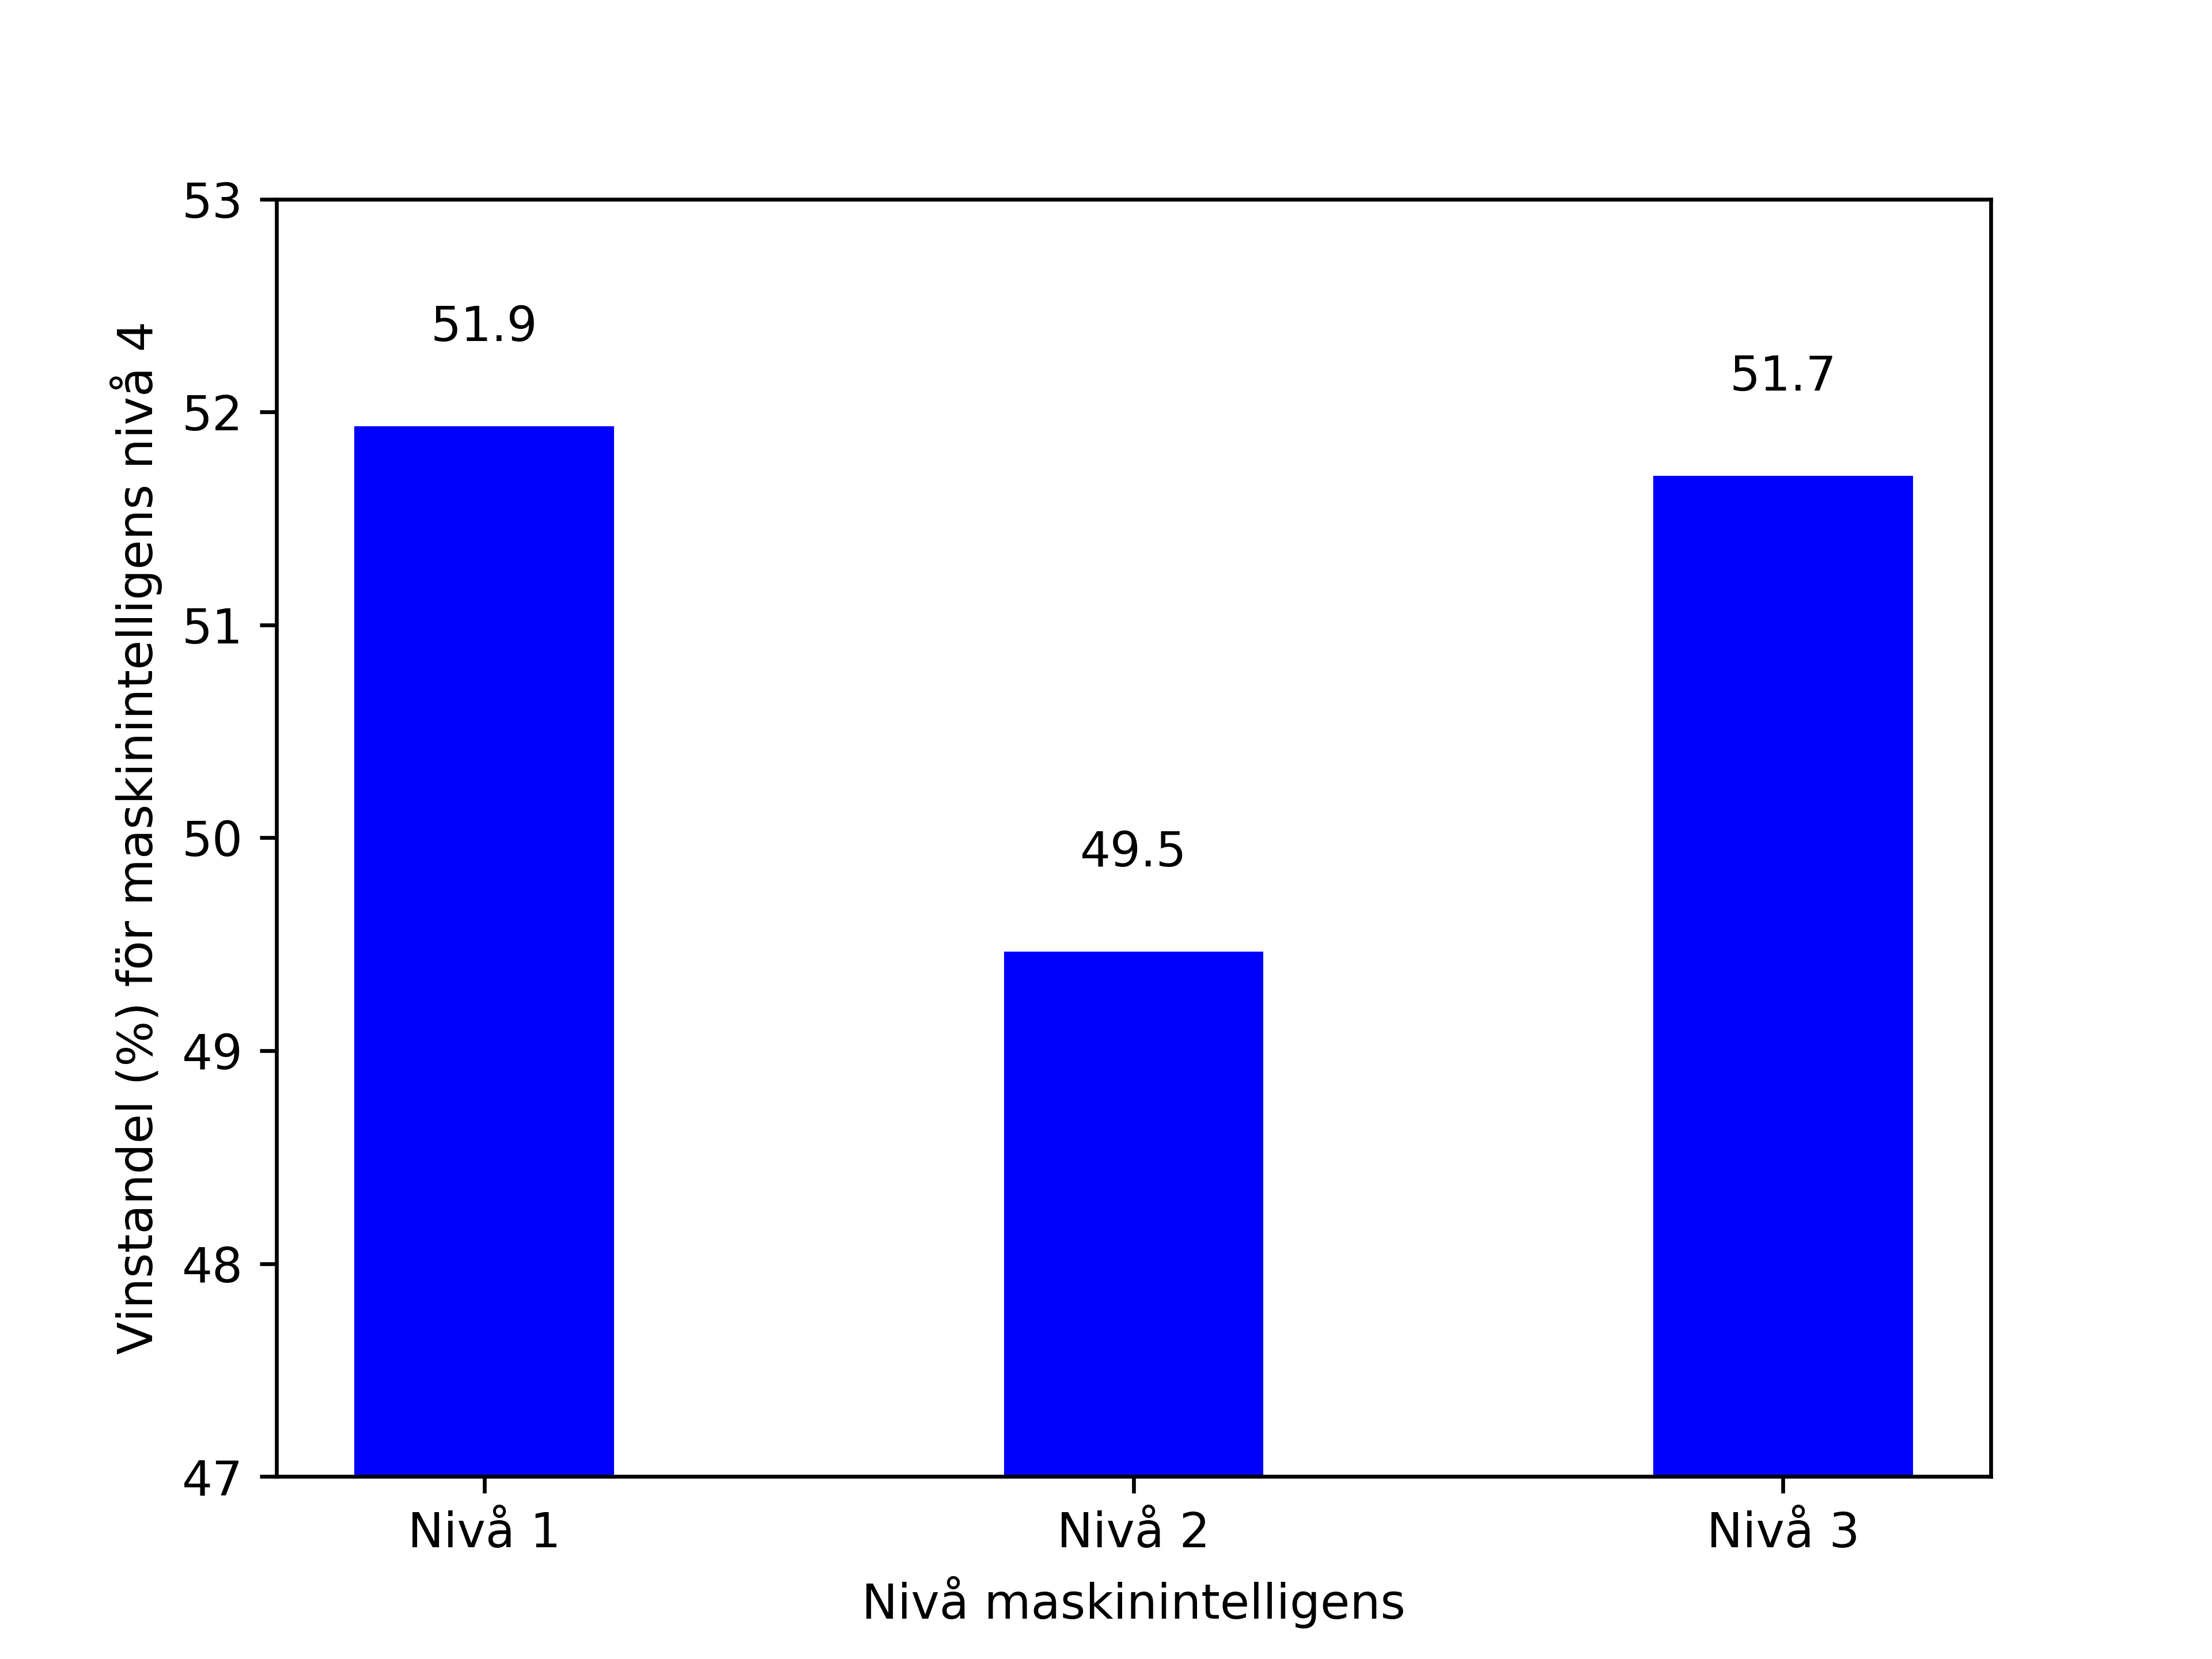
\includegraphics[height=3.5in]{./images/vinstandel_niva4.png}
      \caption{Figuren visar vinstandelen i procent för maskinintelligens
      \emph{nivå 4} då den möter en maskinintelligens av en given nivå.}
      \label{fig:vinstandelniva4} 
    \end{figure}

  \section{Diskussion och slutsats}\label{sec:diskussionochslutsats} 
    Figur 1 visar på att maskinintelligensen ej är bättre än människor på tärningsspelet \emph{Etthundra}. Även om maskinintelligens \emph{nivå 4} vinner flest spel kan ingen slutsats formuleras från denna figur förutom att människor är bättre än maskinintelligensen. Detta då resultatet baseras på en liten mängd spel samt att skillnaden i vinstandel är liten. 
  
    Däremot visar figur \ref{fig:medelpoangmaskinintelligens} på att maskinintelligensen blir bättre då den har tränat fler spel. Detta reflekteras i att medelpoängen maskinintelligensen ackumulerar under ett spels gång tenderar att öka i takt med att maskinintelligensen tränat fler spel. Klart sämst är maskinintelligens \emph{nivå 1} vars medelpoäng är 38,4. Marginellt bäst presterar maskinintelligens \emph{nivå 2}. Denna data är mer tillförlitlig än datan i figur \ref{fig:vinstandelmanniskor} då poängackumulation är mer nyanserat än en vinst eller en förlust, eftersom  ett spel kan förloras med endast 1 poäng eller med 100 poäng. Uppfattningen kring maskinintelligensernas prestation blir således mer detaljerad eftersom analysen av dess poäng medför en större datamängd jämfört med iakttagelser av enbart vinst eller förlust och därför kan figur \ref{fig:medelpoangmaskinintelligens} anses mer tillförlitlig än figur \ref{fig:vinstandelmanniskor}. 

    Figur \ref{fig:vinstandelniva4} förstärker datan i figur \ref{fig:medelpoangmaskinintelligens} då även denna pekar på att maskinintelligens \emph{nivå 2} är den som presterar bäst. Det enda som motsätter sig denna slutsats är figur \ref{fig:vinstandelmanniskor}, där \emph{nivå 4} presterar bäst, men som tidigare nämnts baseras den på minst mängd data och är därför minst tillförlitlig när man ska jämföra de olika nivåerna av maskinintelligens mot varandra. 

    Eftersom maskinintelligensen enbart tränade emot en annan maskinintelligens som hade tränat lika mycket som den själv, lär den sig hela tiden av att spela mot någon som är lika bra, marginellt sämre eller marginellt bättre än sig själv. Detta betyder att den får belöningar för drag och/eller kombinationer av drag som inte skulle lett till en vinst om den mötte en bättre spelare. Maskinintelligensen lär sig därför att spela dåligt, då det räcker med att spela dåligt för att vinna över en sämre motståndare. Det skulle därför vara bättre om maskinintelligensen fick träna mot en väldigt bra motståndare redan från början, och på så sätt lära sig vad som är en bra strategi mot en bra spelare och inte bara mot en dålig. Det bästa hade varit om maskinintelligensen fått träna genom att spela mot människor, eftersom den då lärt sig vad som leder till vinst, men även förlust, vid spel mot just människor. Detta är dock orimligt då maskinintelligensen behöver träna flera miljoner spel för att komma upp i en rimlig nivå. Om man räknar lågt och antar att ett \emph{Etthundra} spel tar en minut att spela och att maskinintelligensen konsekvent kan slå människor efter \emph{1 miljon} tränade spel, skulle det behövas 695 dagars kontinuerligt spelande för att uppnå detta. Ett annat alternativ hade varit att spela mot logik baserat på det optimala sättet att spela \emph{Etthundra}. Då hade maskinintelligensen fått möta en perfekt “spelare” och hade således behövt lära sig att spela på en väldigt hög nivå för att ha en chans att vinna.

    En annan förbättring hade varit att experimentera med $\varepsilon$-värdet. $\varepsilon$-värdet bestämmer hur snabbt stegringen går från att maskinintelligensen slumpmässigt bestämmer alla sina drag under träningen, till att alla dess drag är beräknade. Om detta värdet är för lågt, leder det till att maskinintelligensen slutar att slumpmässigt välja sina drag tidigt och därav utforskas få typer av positioner och dess beräknade drag baseras på en liten mängd data. Maskinintelligensen saknar, med ett lågt $\varepsilon$-värde, erfarenheter och har därför inte tillräckligt med kunskap för att ta bra beslut. Om $\varepsilon$-värdet däremot är för högt kommer maskinintelligensen ta längre tid på sig innan den slutar att välja sina drag slumpmässigt. Detta är egentligen inget dåligt, särskilt inte om maskinintelligensen hela tiden tränar mot en stark motståndare, istället leder enbart ett högt $\varepsilon$-värde till att träningsprocessen tar längre tid. Om det istället är två maskinintelligenser som möter varandra, är ett för högt $\varepsilon$-värde dåligt. Detta då maskinintelligensen och dess motståndare båda kommer att välja sina drag slumpmässigt under en längre tid och dessutom centreras dess inlärning kring slumpmässiga val. Experimentation med $\alpha$ och $\gamma$-värden i SARSA-algoritmen (se \ref{subsubsec:sarsa}) hade även kunnat ge ett bättre resultat, då dessa påverkar i vilken takt maskinintelligensen lär sig. 

  \cleardoublepage

  \section{Källförteckning} \printbibliography[heading=none]

  \section{Källkritik}\label{sec:kallkritik} 
    Alla källor som har använts i denna rapport har valts ut med stor omsorg. Endast förstahandskällor har använts.

    Samtliga artiklar som har nämnts i rapporten är från högt rankade universitet, exempelvis \emph{Massachusetts Institute of Technology}, vilka anses publicera trovärdiga artiklar. Således kan de artiklar som använts anses vara mycket trovärdiga. 

    Den undersökning som rapporten refererat till två gånger är från Stackoverflow, en fråga-svar hemsida för utvecklare. Den är flitigt använd av industrin och är en mycket tillförlitlig källa. Varje år genomför de en undersökning för att ta reda på en rad parametrar och deras undersökningar har alltid många deltagare från hela världen. Detta gör att data från hela världen ackumuleras, vilket ger undersökningen mycket och tillförlitlig data. Således kan undersökningen ses som en mycket trovärdig källa som representerar hela utvecklar-industrin.

  \section{Hållbar utveckling}\label{sec:hallbarutveckling}
    Eftersom maskinintelligenser är beroende av datorer så påverkas miljön negativt eftersom det vid produktionen av datorer sker olika former av miljöfarliga utsläpp. Utöver detta har maskinintelligenser ingen negativ påverkan på miljön och kan istället användas till att förbättra miljön. Ett exempel är förbättring av förbränningsmotorer som nämndes i \ref{sec:inledning}.

  \section{Bilagor}
    \subsection{Q-table - exempel}\label{tab:qtable} 
      \begin{table}[H] \centering 
        \caption{Exempel på hur ett Q-table kan se ut. Värdena är påhittade.} 
        \begin{tabular}{l c r} 
          \textbf{Poäng} & \textbf{Slå} & \textbf{Stanna} \\ 
          \hline 
          40 - 23 - 7    & 30,32        & 10,2 \\ 
          40 - 23 - 12   & 20,74        & 23,12 \\ 
          52 - 46 - 0    & 40,85        & 8,39 \\ 
          52 - 46 - 6    & 32,16        & 13,43 \\ 
        \end{tabular} 
      \end{table} 

      Kolumnen längst till vänster beskriver hur positionen ser ut. Exempelvis beskriver den andra raden (40-23-7) att spelaren har 40 poäng, att motståndaren har 23 poäng och att spelarens temporära poäng är 7. De två andra kolumnerna visar ett värde baserat på hur bra datorn tycker det är att göra respektive drag, slå eller stanna. När datorn utvärderas för att se hur bra den presterar slumpar den ej sina drag utan baserar enbart sina drag på värdena i kolumn två och tre. Exempelvis skulle datorn i positionen 40-23-12 välja att stanna då 23,12 är större än 20,74.

    \subsection{Data och källkod}\label{app:data} 
      Datan och källkoden för denna undersökning ligger uppe på GitHub: \\

      https://github.com/Zelmyx/Gymnasisearbete-Etthundra

\end{document}
